% Preamble
\documentclass[xcolor=dvipsnames]{beamer}
\usetheme{madrid}

% Packages
\usepackage[english,ngerman]{babel}
\usepackage[utf8]{inputenc}
\usepackage{amsmath}
\usepackage{graphicx}
\usepackage{ifthen} % Boolean variables

\definecolor{hBlue}{RGB}{55,118,165}
\usecolortheme[named=hBlue]{structure}

% Distiction between work and stream presentation
\newboolean{work}
\setboolean{work}{false}

\ifthenelse{\boolean{work}}{
    \titlegraphic{
\includegraphics[width=4cm]{../images/logo.png}}
}{}
\title{Gesundheit \& Ernährung}
\ifthenelse{\boolean{work}}{
    \author{Adrian Helberg}
    \date{14.04.2021}
}{
    \subtitle{twitch.tv/bl1nzlar}
    \author{Bl1nzlar}
    \date{\today}
}


% Document
\begin{document}

    \maketitle

    \frame{\frametitle{Agenda}\tableofcontents}

    \section{Theorie}
    {
    \setbeamercolor{normal text}{fg=hBlue}\usebeamercolor*{normal text}
    \begin{frame}
        \begin{center}
            \Huge Theorie
        \end{center}
    \end{frame}
    }

    \subsection{Motivation}
    \begin{frame}[allowframebreaks]
        \frametitle{Motivation}
        \begin{block}{Was ist meine Motivation? Warum der Vortrag?}
            ~
            \begin{itemize}
                \setlength\itemsep{1em}
                \item Gewichtsprobleme im Kindesalter
                \item Starke Gewichtsschwankungen mit langfristiger Zunahme (Jojo-Effekt)
                \item Gescheiterte Versuche abzunehmen
                \begin{itemize}
                    \setlength\itemsep{0.6em}
                    \item Shakes (zB. Almased \textregistered)
                    \item Trennkost
                    \item Kalorienzählen
                    \item Sport
                \end{itemize}
                \item Frust\\~
            \end{itemize}
        \end{block}

        \framebreak

        \begin{itemize}
            \setlength\itemsep{1em}
            \item Warum ist es so schwer das Gewicht zu halten?
            \item Ist der menschliche Körper so dumm, immer weiter krankmachendes Fett anzusetzen?
            \item Liegt es an mir? Was mache ich falsch? Lügen die Medien?
            \item[]
            \item Studium $\rightarrow$ Zugang zur Forschung
        \end{itemize}
    \end{frame}

    \subsection{Die Wissensgesellschaft}
    \begin{frame}[allowframebreaks]
        \frametitle{Die Wissensgesellschaft}
        \begin{figure}
            \centering
            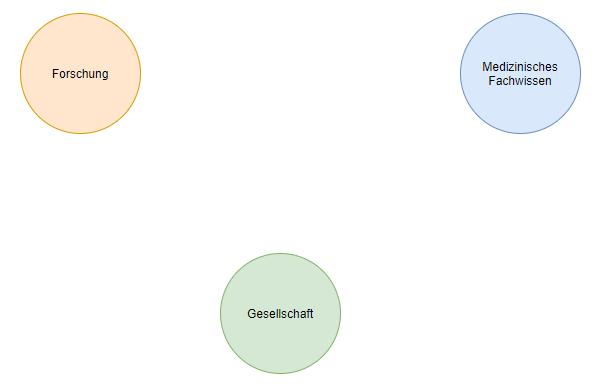
\includegraphics[width=6cm]{../images/wissensgesellschaft_1.png}
            \caption{Forschung und Gesundheit}
        \end{figure}

        \framebreak

        ~\\
        \begin{figure}
            \centering
            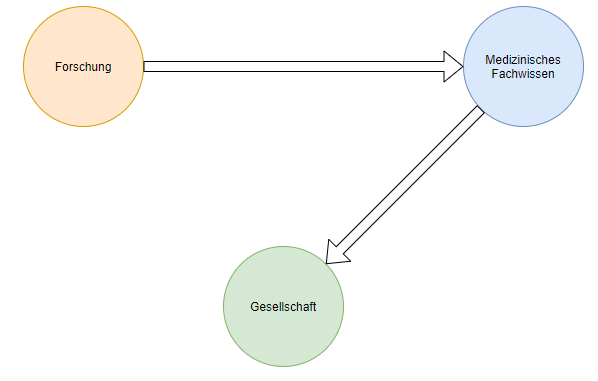
\includegraphics[width=6cm]{../images/wissensgesellschaft_2.png}
            \caption{Informationsfluss}
        \end{figure}

        \begin{figure}
            \centering
            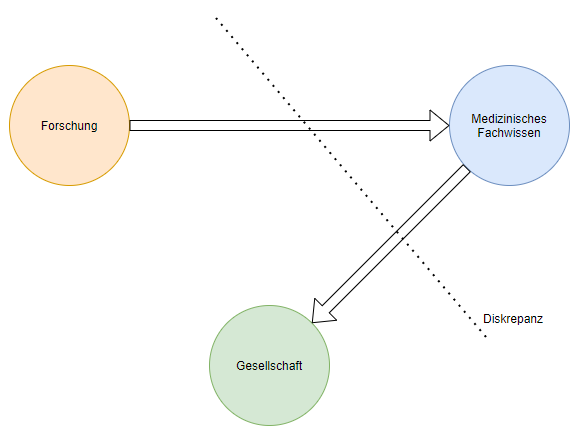
\includegraphics[width=6cm]{../images/wissensgesellschaft_3.png}
            \caption{Diskrepanzen}
        \end{figure}

        \begin{figure}
            \centering
            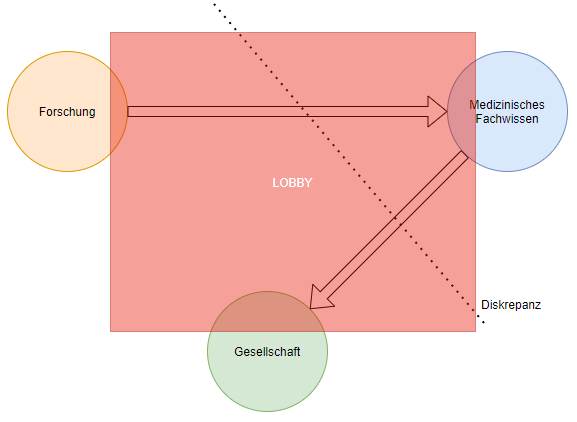
\includegraphics[width=6cm]{../images/wissensgesellschaft_4.png}
            \caption{Lobby}
        \end{figure}

    \end{frame}

    \subsection{Irrtümer}
    \begin{frame}[allowframebreaks]
        \frametitle{Irrtümer}
        \begin{itemize}
            \setlength\itemsep{1em}
            \item Pharma-, Waffen-, Tabak-, Nahrungsmittel-,\\Gesundheits-Industrie, \ldots
            \item 7-Länder-Studie von Ancel Keys 1961
            \item Cholesterien-Lüge 1981
            \item "`Fleisch macht groß und stark"'
        \end{itemize}

        \framebreak

        \begin{figure}
            \centering
            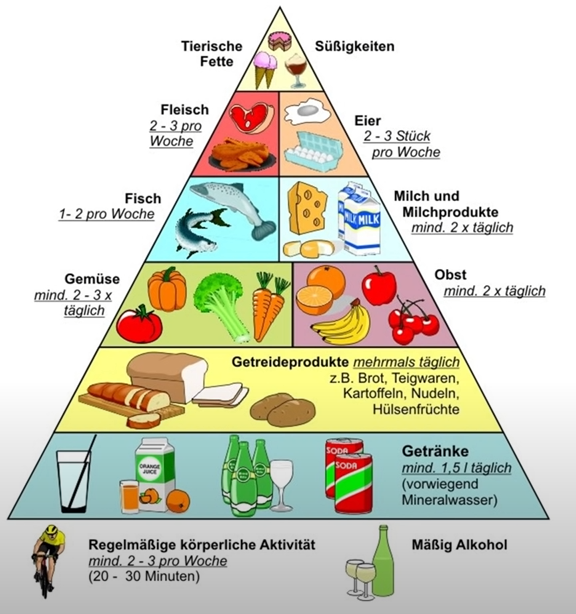
\includegraphics[width=6cm]{../images/pyramide.png}
            \caption{DGE Ernährungspyramide (Deutsche Gesellschaft für Ernährung e.V.)}
        \end{figure}

        \framebreak

        \begin{block}{Weitere Irrtümer...}
            \begin{itemize}
                \setlength\itemsep{1em}
                \item "`Dünn zu sein ist gesund"'
                \item "`Die Gene sind schuld"'
                \item "`Fett macht fett"'
                \item "`Essen hat nichts mit Hormonen zu tun"'
                \item "`Nur die Kalorienbilanz zählt"'
                \item "`Ich bin zu willensschwach"'
                \item "`Rauchen hält schlank"'
                \item "`Gewichtsprobleme sind überbewertet"'
            \end{itemize}
        \end{block}
    \end{frame}

    \subsection{Hunger}
    \begin{frame}[allowframebreaks]
        \frametitle{Hunger}
        \begin{block}{Was passiert dann?}
            \begin{itemize}
                \setlength\itemsep{1em}
                \item[1.] Kohlenhydratzufuhr
                \item[2.] Verdauung $\rightarrow$ Zuckertsunami im Blut (Blutzuckeranstieg)
                \item[3.] Zucker "`verzuckert"' Eiweißmoleküle $\rightarrow$ Panikreaktion des Körpers
                \item[4.] Maximale Insulinproduktion $\rightarrow$ Zucker wird für den Energiebedarf bereitgestellt oder
                bei gedecktem Bedarf in die Zellen gebracht
                \item[5.] Glucagonausschüttung durch niedrigen Blutzuckerspiegel\\(leider zu langsam\ldots)
                \item[6.] Erneut Hunger nach 2 Stunden
            \end{itemize}
        \end{block}

        \framebreak

        \begin{block}{Warum will der Körper diese Nahrungsmittel?}
            \begin{itemize}
                \setlength\itemsep{1em}
                \item Kopfhunger,   Stichwort: Sinneswahrnehmung
                \item Zellhunger,   Stichwort: Energieversorgung
                \item Bauchhunger,  Stichwort: Mikrobiom
                \item Herzhunger,   Stichwort: Serotonin
            \end{itemize}
        \end{block}
    \end{frame}

    \subsection{Fazit}
    \begin{frame}
        \frametitle{Fazit}
        \begin{center}
            \textbf{Fett ist \underline{nicht} das Problem, sondern die Lösung!}
        \end{center}
    \end{frame}

    \subsection{Ziel}
    \begin{frame}
        \frametitle{Ziel}
        \begin{block}{Wie schaffen wir es gesund zu werden / bleiben?}
            Erreichen einer ganzheitlichen Zellgesundheit durch einbeziehen morderner Ernährungswissenschaften mit
            \begin{itemize}
                \item passender Ernährungsform
                \item Erkennen krankmachender Verhaltensmuster bei Lebensstil, Bewegung und Schlaf
                \item Reparatur des Mikrobioms im Darm
            \end{itemize}
        \end{block}

        \textit{So schaffen wir es den Körper peu á peu auf schlank umzuprogrammieren}

    \end{frame}

    \section{Praxis}
    {
        \setbeamercolor{normal text}{fg=hBlue}\usebeamercolor*{normal text}
        \begin{frame}
            \begin{center}
                \Huge Praxis
            \end{center}
        \end{frame}
    }

    \subsection{Das perfekte Frühstück}
    \begin{frame}[allowframebreaks]
        \frametitle{Das perfekte Frühstück}
        \underline{Rezept}:
        \begin{itemize}
            \setlength\itemsep{0.6em}
            \item 3 EL Magerquark
            \item 3 EL Naturjoghurt
            \item 1 EL Leinöl
            \item 1 EL Weizenkeimöl
            \item Saft einer halben Zitrone
            \item 1 EL Leinsamenschrot
            \item Verschiedene Nüsse
            \item 1 TL Zimt
            \item 1 TL Kurkuma
            \item Eine Hand voll Beeren (Tipp: TK Beerenmix)
        \end{itemize}

        \framebreak

        \begin{block}{Wichtig}
            \begin{itemize}
                \setlength\itemsep{1em}
                \item Öle kalt und dunkel lagern (Kühlschrank)
                \item Nüsse am besten mit Schale, kalt und dunkel lagern (Kühlschrank)
            \end{itemize}
        \end{block}

    \end{frame}

    \subsection{Das Spätstück}
    \begin{frame}
        \frametitle{Das Spätstück}
        \begin{itemize}
            \setlength\itemsep{1em}
            \item Die Pause zur Selbstheilung (Autophagie)
            \item 15 Stunden Fasten (bspw. 18:00 - 09:00)
        \end{itemize}
    \end{frame}

    \section{Fragerunde}
    {
        \setbeamercolor{normal text}{fg=hBlue}\usebeamercolor*{normal text}
        \begin{frame}
            \begin{center}
                \Huge Fragerunde
            \end{center}
        \end{frame}
    }

\end{document}
